\chapter{Physical Terminology}

\section{anisotropy}
各向异性或非均向性,指物体的全部或部分属性性质随方向的不同有不同的变化

在计算机图形学中,各向异性表面在围绕几何法线旋转时外观会发生变化。

任何具有细粒度的东西,会产生影响外观的作用。

\subsection{anisotropy reflect}
基于反射表面上存在的小凹槽或凸起,改变光源照射物体的方向,反射在各个方向上具有不同的特性。

可用来平滑图像,克服高斯模糊的缺陷。

\subsection{isotropy reflect}
表面反射均匀具有模糊效果, 反射总是在与颗粒相反的方向拉伸。

\section{Light}

\subsection{Conception}

\subsubsection{Absorption \& Scattering}

吸收与散射, 当光在一个不均匀介质中或半透明的材质中传播时,会被吸收或散射。

\subsection{Refraction}

\subsubsection{IOR}
index of refraction,折射率,光在真空中的传播速度与光在介质中的传播速度之比。
折射率与介质的电磁性有关,

\paragraph{绝对折射率}

光在某种介质中的速度为v,真空中的光速为c,则介质的绝对折射率为$n=\frac{c}{v}$

\paragraph{相对折射率}

光从介质1射入介质2发生折射时,入射角$\theta_{1}$与折射角$\theta_{2}$的正弦之比$n_{21}$
叫做介质2相对介质1的折射率。
\begin{align*}
    n_{1} \cdot sin(\theta_{1}) &= n_{2} \cdot sin(\theta_{2}) \\
    n_{21} &= \frac{n_{2}}{n_{1}}
\end{align*}

\paragraph{全反射}

光由相对光密介质射入相对光疏介质,且入射角大于等于临界角C。临界角是指入射角满足折射角为$90^{\circ}$。
\begin{align*}
    \frac{n_{1}}{n_{2}} = \frac{sin90^{\circ}}{sinC}
\end{align*}
空气的折射率是$n_{2}=1$, 则介质向空气入射可简化为$n=1/sinC$.

\paragraph{光色散}

对不同的波长,介质的折射率$n(\lambda)$不同,这叫做光色散.

\subsection{Reflectance}

反射率,是用来衡量物质反射能力的量,定义为物体表面反射能量与达到物体表面入射能量的比率。反射率是波长的函数,
指某段波长向一定方向的反射,不同波长就有不同的反射率。
\begin{align*}
    \phi(\lambda) = \frac{E_{R}(\lambda)}{E_{I}(\lambda)} = \frac{\pi L(\lambda)}{E_{I}(\lambda)}
\end{align*}

\subsection{Albedo}

反照率,指地表在太阳辐射的影响下,反射辐射通量与入射辐射通量的比值。albedo是对全波段的,是反射率在所有方向上的积分。

\begin{align*}
    \alpha = \frac{M}{E}
\end{align*}

\subsubsection{White Sky Albedo}

WSA,白空反照率,指忽略太阳直射辐射,只考虑地物对大气散射辐射的反射情况。

\subsubsection{Black Sky Albedo}

BSA,黑空反照率。指忽略大气散射,只考虑地物对太阳直射,入射,辐射的反射情况

\subsubsection{Blue Sky Albedo}

地物真实反照率,又称为蓝空反照率,或半球-半球反射率BHR

\begin{align*}
    BHR \approx (1-s)WSA + sBSA 
\end{align*}

其中s是天空散射光比例。

\subsection{辐射学}

\begin{center}
    \begin{tabular}{|c|c|c|c|c|} \hline
       \hbox{名称} & \hbox{单位} & \hbox{符号} & \hbox{对应色度单位} & \hbox{色度单位} \\ \hline
       \hbox{Radiant energy/辐射能} & \hbox{焦耳Q} & \hbox{Q} & \hbox{Luminous energy光能量}  & \hbox{tblbot} \\ \hline
       \hbox{Radiant flux辐通量} & \hbox{瓦特W} & \hbox{$\Phi$} & \hbox{Luminous flux光通量}  & \hbox{流明lm} \\ \hline
       \hbox{Intensity/辐强度} & \hbox{W/sr} & \hbox{I} & \hbox{Luminous intensity光出射度}  & \hbox{坎德拉cd=lm/sr} \\ \hline
       \hbox{Irradiance辐照度} & \hbox{$W/m^{2}$} & \hbox{E} & \hbox{Illuminance发光强度}  & \hbox{勒克斯$lx=lm/m^{2}$} \\ \hline
       \hbox{Radiance辐亮度} & \hbox{$W/(m^{2}sr)$} & \hbox{L} & \hbox{Luminance光亮度}  & \hbox{尼特$nit=lm/(m^{2}sr)$} \\ \hline
    \end{tabular}
\end{center}

\paragraph{辐射能}
energy,$Q_{e}$单位是焦耳$J$,单个光子的辐射能表示为$Q=\frac{nc}{\lambda}$

\paragraph{辐通量}
flux, $\Phi_{e}$,单位时间内发射,接收或传输的能量$\Phi_{e}=\frac{dQ}{dt}$,单位是瓦特W.

\paragraph{辐照度}
irradiance辐照度$E_{e}$, radiant exitance辐出度$M_{e}$,辐照度表示单位面积受到的辐通量$E_{e}=\frac{d\Phi}{dA}$, 
辐出度表示单位面积发出的辐通量$M_{e}=\frac{d\Phi}{dA}$,单位都是$W/m^{2}$,辐通量为$\Phi$的点光源在距离r处球面上的辐照度
为$E_{e}=\frac{\Phi}{4 \pi r^{2}}$.

\paragraph{辐强度}
radiant intensity$I_{e}$,元立体角内的辐通量$I_{e}=\frac{d\Phi}{d\Omega}$,单位是$W/sr$

\paragraph{立体角}
solid angle可以看作平面角在球体上的扩展,单位是球面度$sr$,整个球面的总立体角是$4\pi$,半球面的总立体角和是$2\pi$

\paragraph{辐亮度}
radiance, $L_{e}$表示单位面积和单位立体角上的辐通量$L_{e}=\frac{d^{2}\Phi_{e}}{dA^{T}d\Omega}=\frac{d^{2}\Phi_{e}}{cos\theta dA d\Omega}$,
单位是$W/(m^{2}\dot sr)$,辐亮度是用来描述传感器(摄影机,人眼等)感受辐射最常用的量,也是最重要的量。

\subsection{光度学}

辐射的度量是纯物理的方式来描述的,而人眼只能看到波长在400nm~700nm波长的电磁波,所以要转换为描述人眼感知的光学度量,就是
\textbf{光通量}$\Phi_{v}$,单位流明lm,\textbf{光照度}$E_{v}$,单位勒克斯$lx=\frac{lm}{m^2}$,\textbf{发光强度}$I_{v}$单位坎德拉
$cd=\frac{lm}{sr}$,\textbf{光亮度}$L_{v}$,单位$nit=\frac{cd}{m^2}$.

光在不同的波长上的分布,叫做光谱功率分布spectral power distributions(SPD)。人眼作为一种探测器,输入是辐射量表示的可见光辐射,输出的是感受值的光学量。
它们之间的关系可表示为$\Phi_{v}=683.002(lm/w) \cdot \int_{0}^{\infty}{\bar{y}(\lambda)\Phi_{e,\lambda}(\lambda)d\lambda}$, 其中$\Phi_{e,\lambda}$
是光谱功率分布,单位是$W/nm$;$\bar(y)$是光度函数,没有单位;$\lambda$是波长,单位是nm。

所有渲染公式中用到的都是光度学单位,而描述看到的颜色的最终结果的单位是$cd/m^2$。鉴于点光源和平行光源的不同特性,使用不同的单位来描述的,
点光源用\textbf{发光强度I},单位是cd;而平行光源用\textbf{光照度E},单位是lx。,对点光源S,距离r的光照度为$E=\frac{d\Phi}{dA}=\frac{I}{r^2} \cdot 1sr$.

\section{CIE}

自然界真实的光照有很复杂的SPD,但人眼的颜色感受细胞只有三种,分布是红绿蓝RGB三种,即可以将复杂的光谱功率分布转换为RGB表示。

CIE-RGB标准,指定三原色r(645nm), g(526nm), b(444nm)的光谱映射函数和SPD求内积,将一个任意的SPD表示为三个刺激值。
这种方式得到的值有负值,不便于计算,在CIE-RGB基础上改进为CIX-XYZ,将SPD$s(\lambda)$通过求内积转换成三个刺激值XYZ:

\begin{align*}
    X = \int_{380}^{780}s(\lambda)\bar{x}(\lambda)d\lambda, \newline
    Y = \int_{380}^{780}s(\lambda)\bar{y}(\lambda)d\lambda, \newline
    Z = \int_{380}^{780}s(\lambda)\bar{z}(\lambda)d\lambda
\end{align*}

其中$\bar{y}(\lambda)$的曲线就是计算光度学量的光度函数,即Y值可以作为颜色的亮度值。

为了把颜色的亮度和色度区分开,定义

\begin{align*}
    x = \frac{X}{X+Y+Z}, \newline
    y = \frac{Y}{X+Y+Z}, \newline
    z = \frac{Z}{X+Y+Z} = 1 -x - y
\end{align*}

利用上面公式,用xy的值绘制成一张图,得到CIE色品图,是1931 Color Space。图中范围就是人眼可见光范围,
边缘的曲线表示纯色,对应着光谱值,中心点代表D65纯白色。在图中任意取一颜色点,与中心点的延长线交于曲线处的
颜色叫做\textbf{色相hue},中心点与颜色点的距离与中心点延长交于曲线的距离的比值叫\textbf{饱和度saturation}。
从色品图中取一个颜色点,加上亮度值,就构成CIE-XYZ坐标系统来描述任意颜色。

\begin{figure}[h]
    \centering
    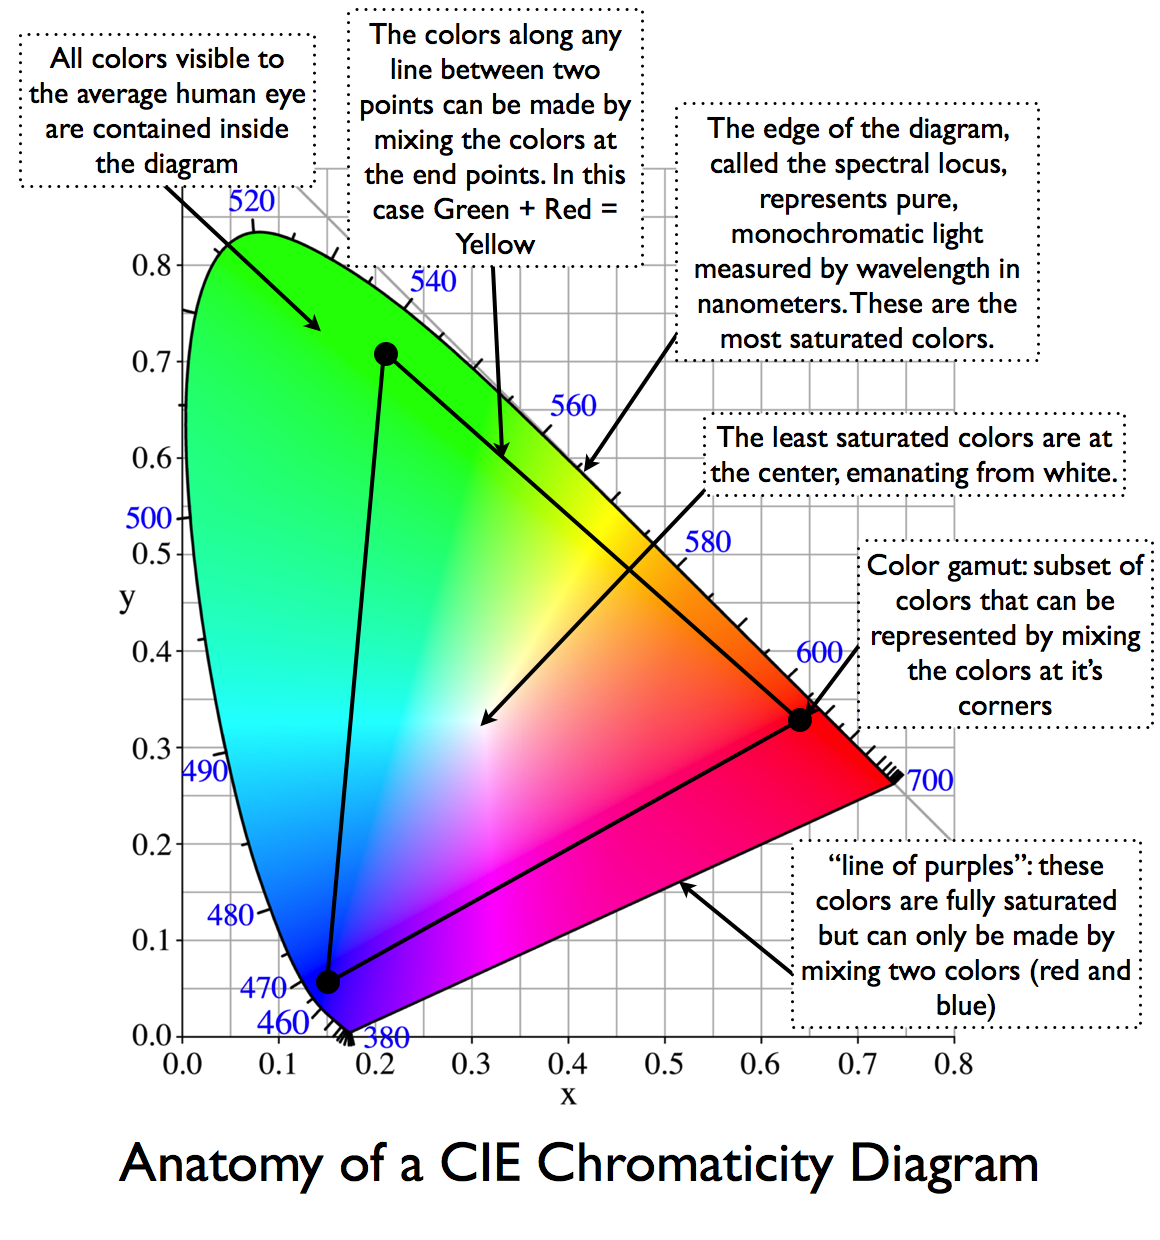
\includegraphics[width=1\textwidth]{images/anatomy-of-a-cie-1931-color-space.png}
\end{figure}

选取三个点作为纯色RGB颜色,形成一个三角形\textbf{色域gamunt},色域中的颜色可以任意进行线性混合。RGB色域有很多种,
,图中三个黑色点就是sRGB色域,还有Adobe 1998色域;DCI-P3苹果系列产品使用的色域;ACEScg一种设计用来计算渲染的色域。
\textbf{色品图中的色域只是一个投影,真实的色域应该是一个立体形的,包括亮度值}。

从RGB色域到XYZ三刺激值的互相转换是线性的,可以用矩阵来表示。如sRGB色域中,有$Y = 0.2126R + 0.7156G + 0.0722B$,Y就是
亮度值,在实时渲染中常用来计算亮度来模拟自动曝光的一个参数。RGB色域并不真实反映物体对光SPD的反馈,但除少数工业级电影的离线渲染
使用频谱渲染,其他都可以满足要求了。

\subsection{伽马校正}

早期的CRT显示器的输入电压和显示亮度并不是线性关系,是$I=V^{2.2}$的非线性关系,显示器的显示亮度和输入值的关系称为
\textbf{EOTF(electrical optical transfer function)},由硬件层实现自动转换。

实时渲染中的颜色值计算都是在线性空间中,为了让显示器正确显示颜色,需要在Framebuffer中进行伽马校正,来抵消EOTF的效果。

人眼对亮度的感受会随着亮度的增高而减弱,如果是线性编码,人眼对低亮度的变化更加敏感,如果使用8bit(0~255)的线性编码颜色,
就会产生很严重的色差。对线性的sRGB进行一次伽马校正后,这样就可以直角显示了,目前大部分图片的格式都经过sRGB伽马校正了。

可是渲染时,从图片中获取的像素值是经过伽马校正的,需要转换为线性空间的sRGB,以便于渲染计算的正确性。最后在FrameBuffer阶段
还是需要进行伽马校正的来保证显示器正确显示最终的色值。

\subsection{HDR - Tone Mapping}
hight dynamic range在渲染和硬件中的两种意思,这里指渲染的意思。

随着PBR渲染及硬件的发展,渲染计算中的光照值的范围需要转换成显示器中的显示范围,这个映射的过程叫做\textbf{Tone Mapping}。
尽可能还原图像的细节,而不仅仅线性的缩放,tone mapping映射为曲线时能保留亮部和暗部的细节。

\subsection{EV100}

计算图像的整体平均亮度是必须的,一般采用log平均的方式

\begin{itemize}
    \item {传统方式是算出图像的亮度log值后,不断DownSample直到一个1x1的texture,即可算出图像的平均亮度}
    \item {现代使用Computer Shader,统计每个亮度范围的像素点数,再综合计算得到一个亮度值}
\end{itemize}

EV(exposure value)在摄影中表示需要曝光值,EV100表示在ISO100标准下的EV值和光亮度的关系,$EV_{100}=log_{2}(\frac{E}{0.78} \cdot q)$
,$q$表示光在光学系统中传递时的损耗,游戏引擎中是一个模拟值,取$q=0.65$。

\chapter{Physical Simulation}

\section{Material Point Method}

物质点法,是一种模拟连续介质的方法,最早被Sulkey等人在1995年发明。
与有限元相比,可以把MPM里面的grid nodes对应到FEM中的DOFs,
把MPM里面的particles对应到FEM中的quadrature points。和FEM里使用显式网格策略
不同,作为一种Element-Free Galerkin(EFG)方法,MPM里面并没有显式的Elements
和Lagrangian grid,只有能够随意移动的粒子,作为quadrature points。这样的特性
非常适合处理大形变,而其背景网格带来的自动碰撞处理,多材料耦合等。由于离散化
出自weak form,使得MPM的physical accuracy有了保证。

\subsection{Moving Least Squares Material Point Method}

移动最小二乘物质点法,

\chapter{Physically Based Rendering}

Physically Based Rendering Toolkit是一个基于物理渲染的开源离线渲染器, 可参考配套的书\cite{PBR3ed}。



\paragraph{Markov Process}

Markov Chain可应用到渲染上是基于Detailed Balance的方法。

光线传递的随机性(光子抵达物体表面材质后被吸收或随机反射)仅由当前状态决定,和历史无关,满足马可夫过程定义。

在渲染中使用Markov Chain Monte Carlo没有复杂的物理,现代所有光线传播的模拟都是基于对渲染方程rendering equation
的求解,而渲染方程已经将原本的物理系统大大的简化了,所以光线传递的物理到底是不是平稳马尔可夫过程和渲染没有任何关系,
渲染只是要计算一个定义域纬度很高的函数而已,对于一个场景,固定的一组输入是会返回一个固定的值,没有什么随机和模糊的东西,
最极端简化就是一个一维函数,Metropolis Sampling的牛逼之处在于它不需要求解函数的积分或者算它的概率分布就能给你提供一系列
和目标高数概率分布一致的样本,这一点对基于Monte Carlo的渲染来说十分重要,叫做重要性采样Importance Sampling。

所以Metropolis Sampling主要用来渲染一些采样路径特别复杂的场景,一般室外大太阳的场景用不着付出额外的计算。Metropolis Light Transport
的论文就是用了一个光源在一个微微打开的门缝后面的场景当例子。
